\subsection{Memoria de Algoritmos de Sorting}

El análisis experimental de la memoria confirma las cotas asintóticas y exhibe el peso de las estructuras de datos auxiliares. Teóricamente, \textsc{QuickSort} y \textsc{sort} son algoritmos \emph{in-place} con espacio auxiliar en la pila de recursión de $O(\log n)$; \textsc{MergeSort} no es \emph{in-place} al requerir un arreglo temporal continuo de dimensión idéntica a la entrada ($\Theta(n)$); y \textsc{PatienceSort} almacena la totalidad de los datos en pilas intermedias, conservando una cota espacial de $O(n)$.

\begin{figure}[H]
    \centering
    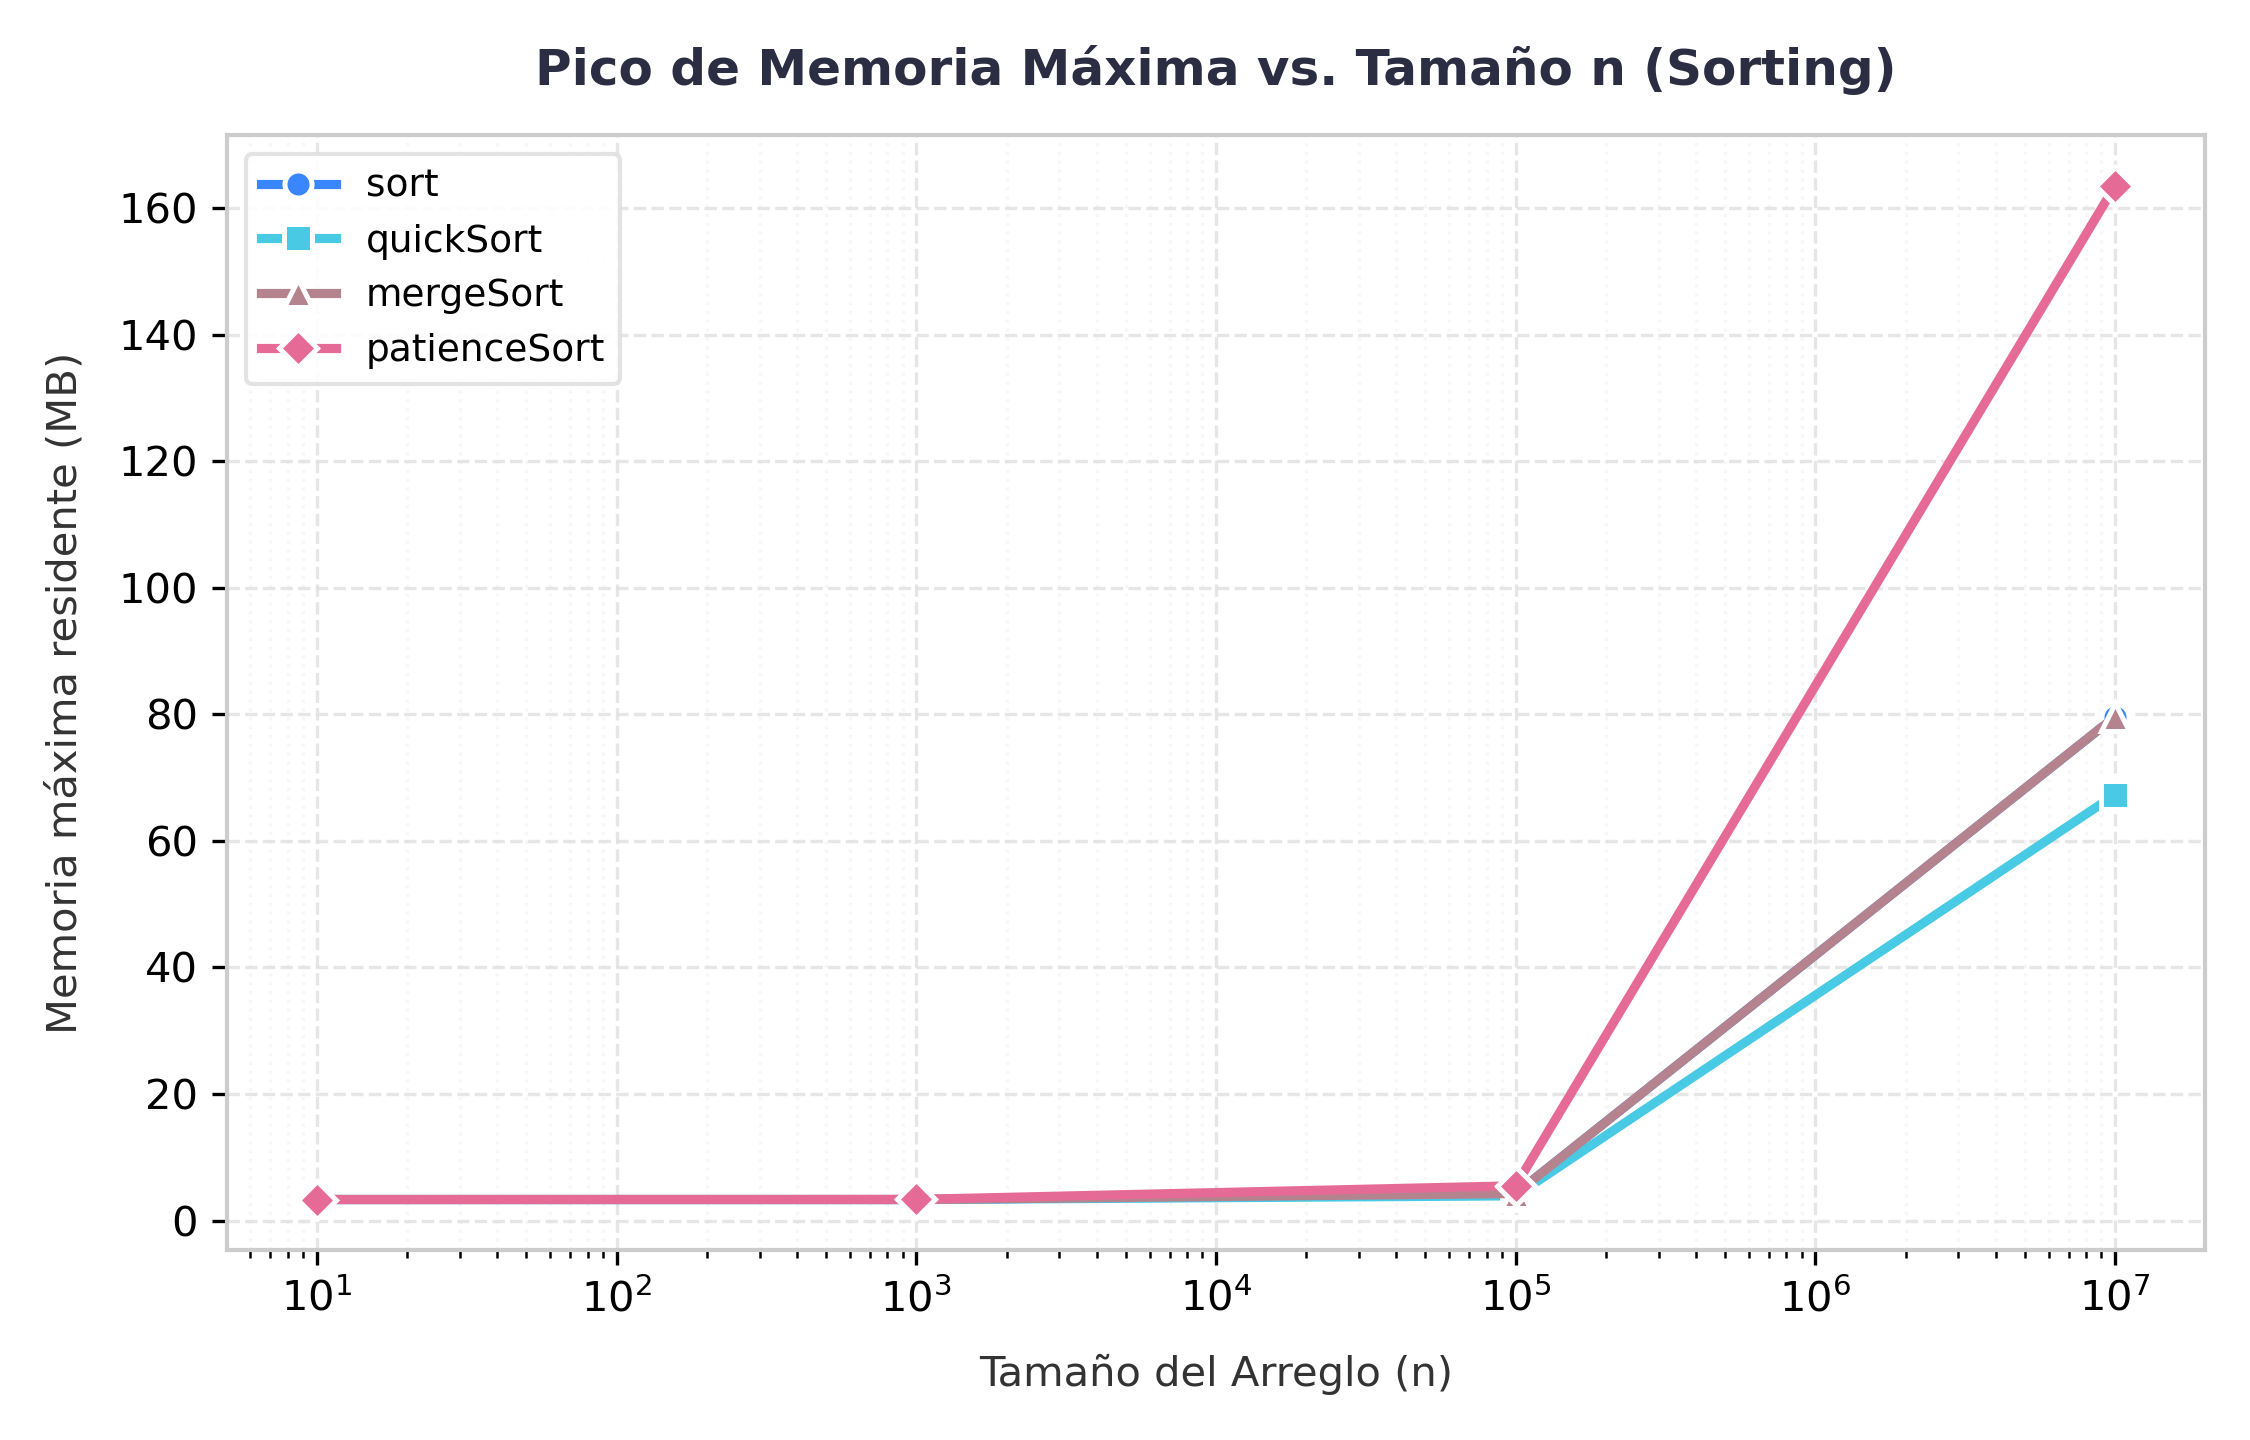
\includegraphics[width=0.72\linewidth]{../code/sorting/data/plots/memoria_sorting.png}
    \caption{Pico de memoria máxima vs. tamaño del arreglo $n$ en algoritmos de ordenamiento.}
    \label{fig:sort_mem}
\end{figure}

Como se aprecia en la \Cref{fig:sort_mem}, el consumo de memoria se mantiene bajo y uniforme para todos los algoritmos en dimensiones pequeñas ($n \le 10^5$), disparándose de forma notoria al alcanzar $n = 10^7$. En esta escala, \textsc{PatienceSort} resulta ser el método menos eficiente: aunque su cota asintótica de datos es lineal $O(n)$, la representación en C++ mediante vectores dinámicos anidados aumenta el consumo de memoria respecto al resto. Por su parte, \textsc{QuickSort} se posiciona en el extremo más eficiente al operar directamente sobre el arreglo original. Finalmente, \textsc{sort} y \textsc{MergeSort} se ubican en una franja intermedia muy próxima entre sí; mientras que en \textsc{MergeSort} esto concuerda con la reserva física de su vector auxiliar $\Theta(n)$, en \textsc{sort} responde a la memoria base del proceso y a las asignaciones internas del entorno en tiempo de ejecución.

\subsection{Tiempo de Ejecución de Algoritmos de Sorting}

En el plano temporal, \textsc{sort} garantiza $O(n \log n)$ en el peor caso; \textsc{QuickSort} exhibe un caso promedio de $O(n \log n)$ con peor caso $O(n^2)$; \textsc{MergeSort} presenta una complejidad estricta de $\Theta(n \log n)$ en todos los escenarios; y \textsc{PatienceSort} posee una complejidad adaptativa de $O(n \log p)$, donde $p$ denota la cantidad de pilas formadas ($1 \le p \le n$), fluctuando entre $O(n)$ en el mejor caso y $O(n \log n)$ en el peor caso.

\begin{figure}[H]
    \centering
    \subfloat[Arreglos aleatorios.\label{fig:sort_time_aleatorio}]{%
        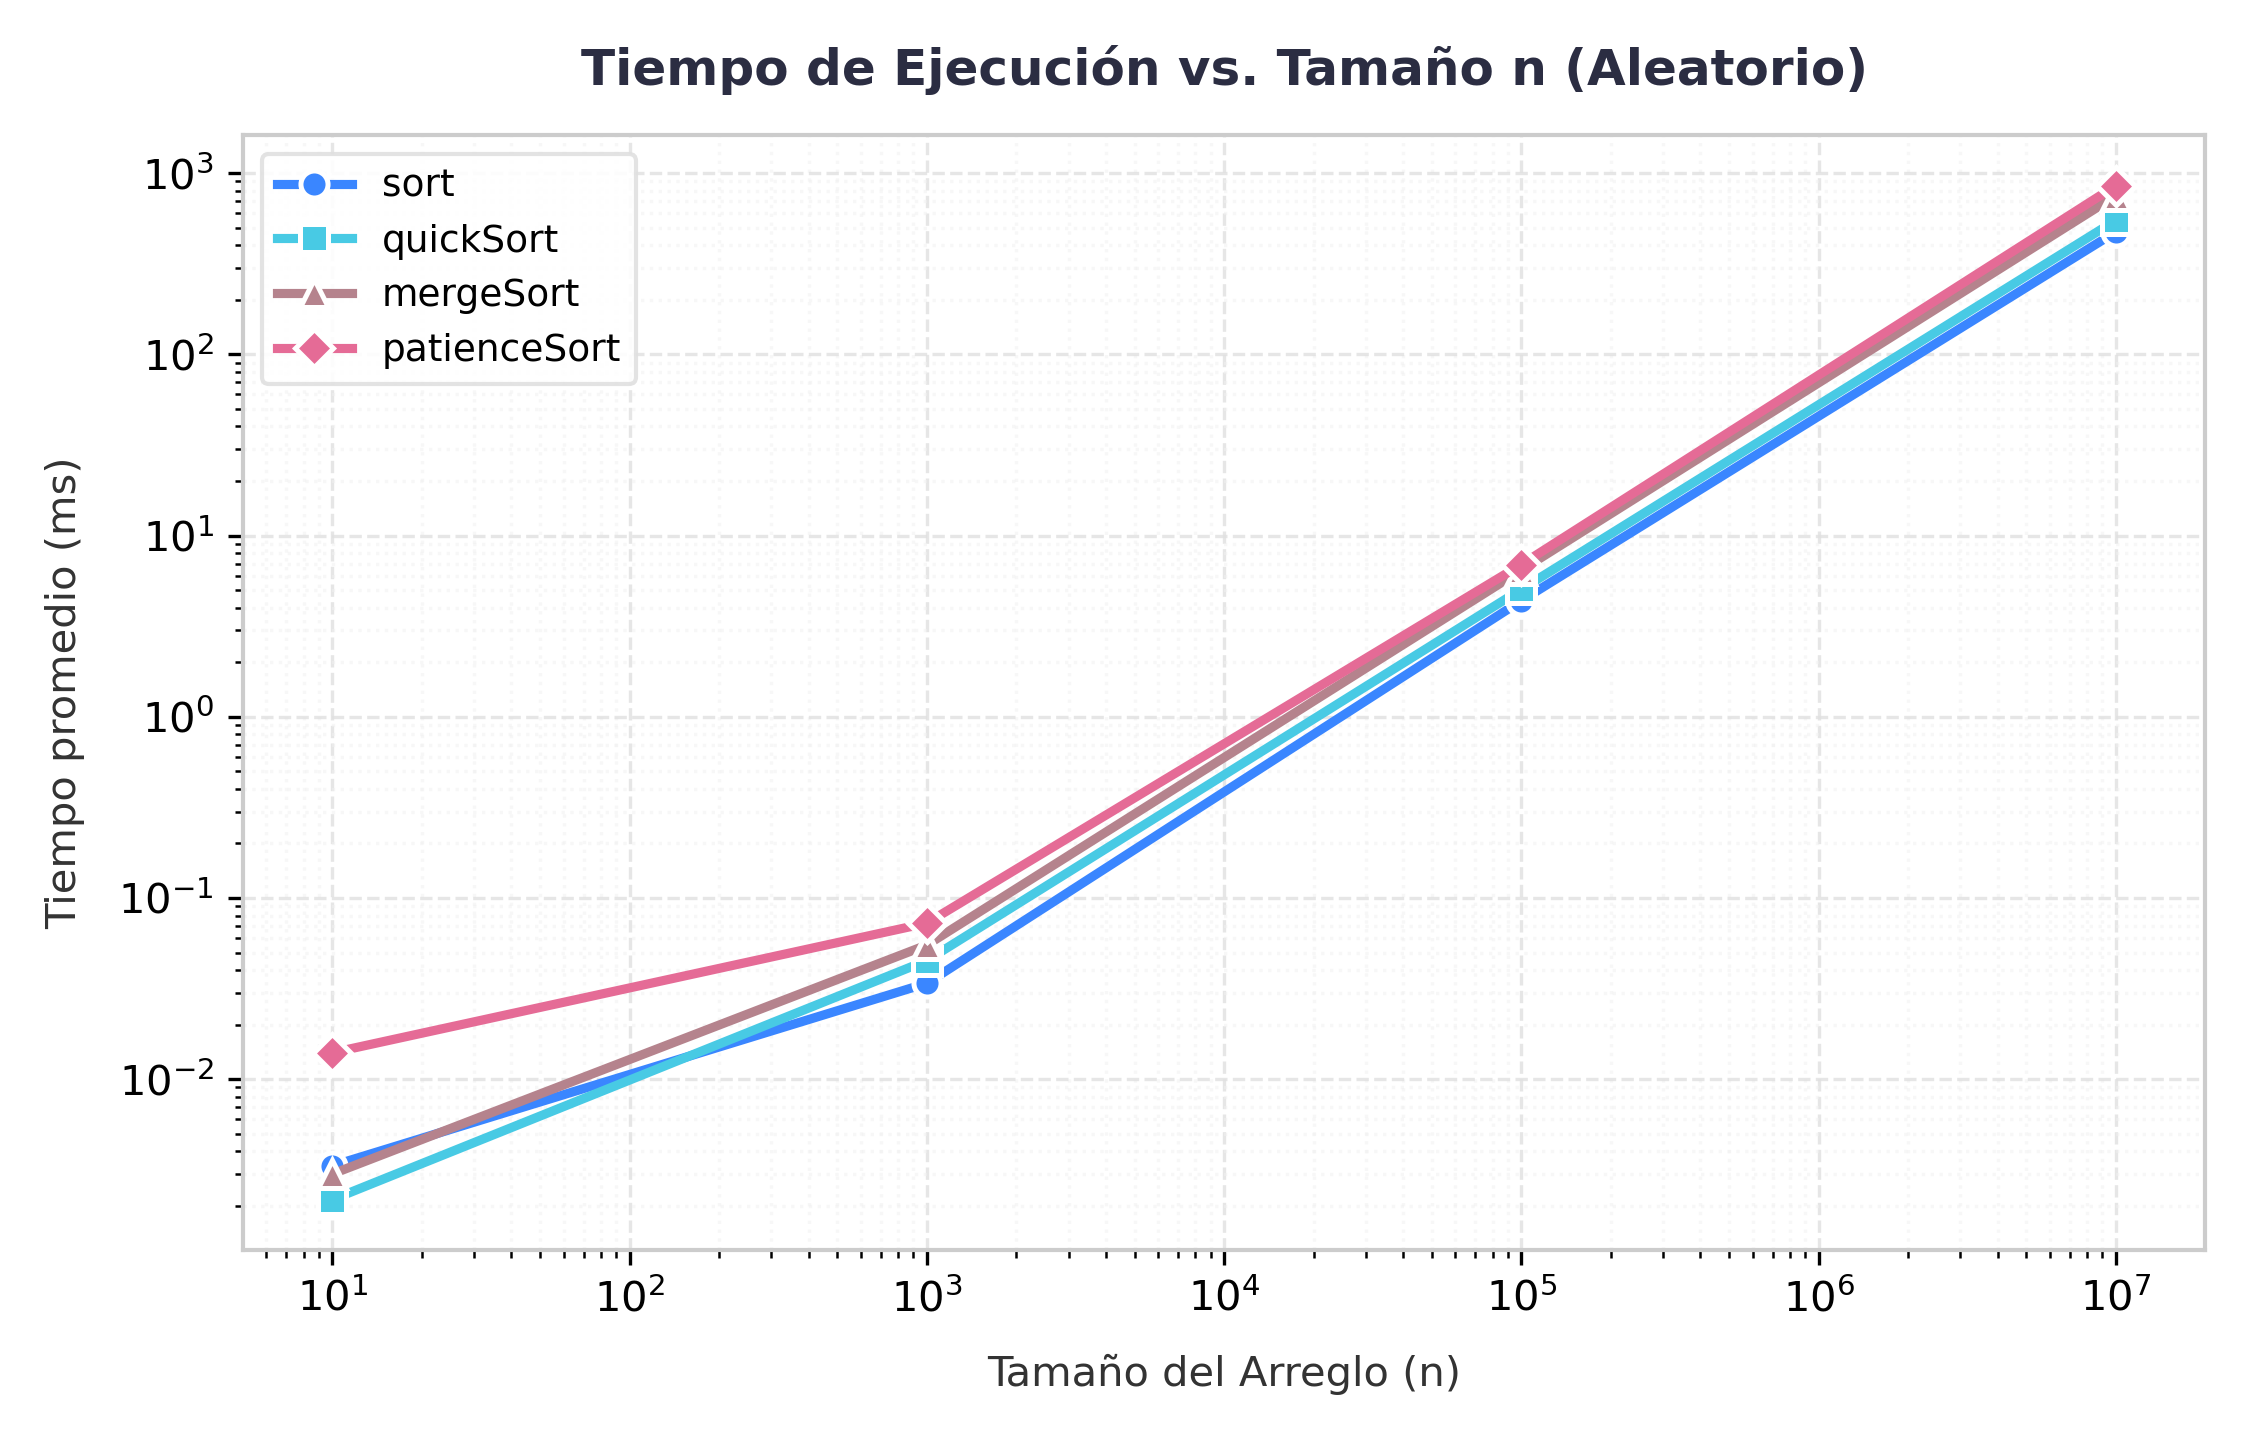
\includegraphics[width=0.48\linewidth]{../code/sorting/data/plots/tiempo_sorting_aleatorio.png}%
    }
    \hfill
    \subfloat[Arreglos ordenados ascendentemente.\label{fig:sort_time_ascendente}]{%
        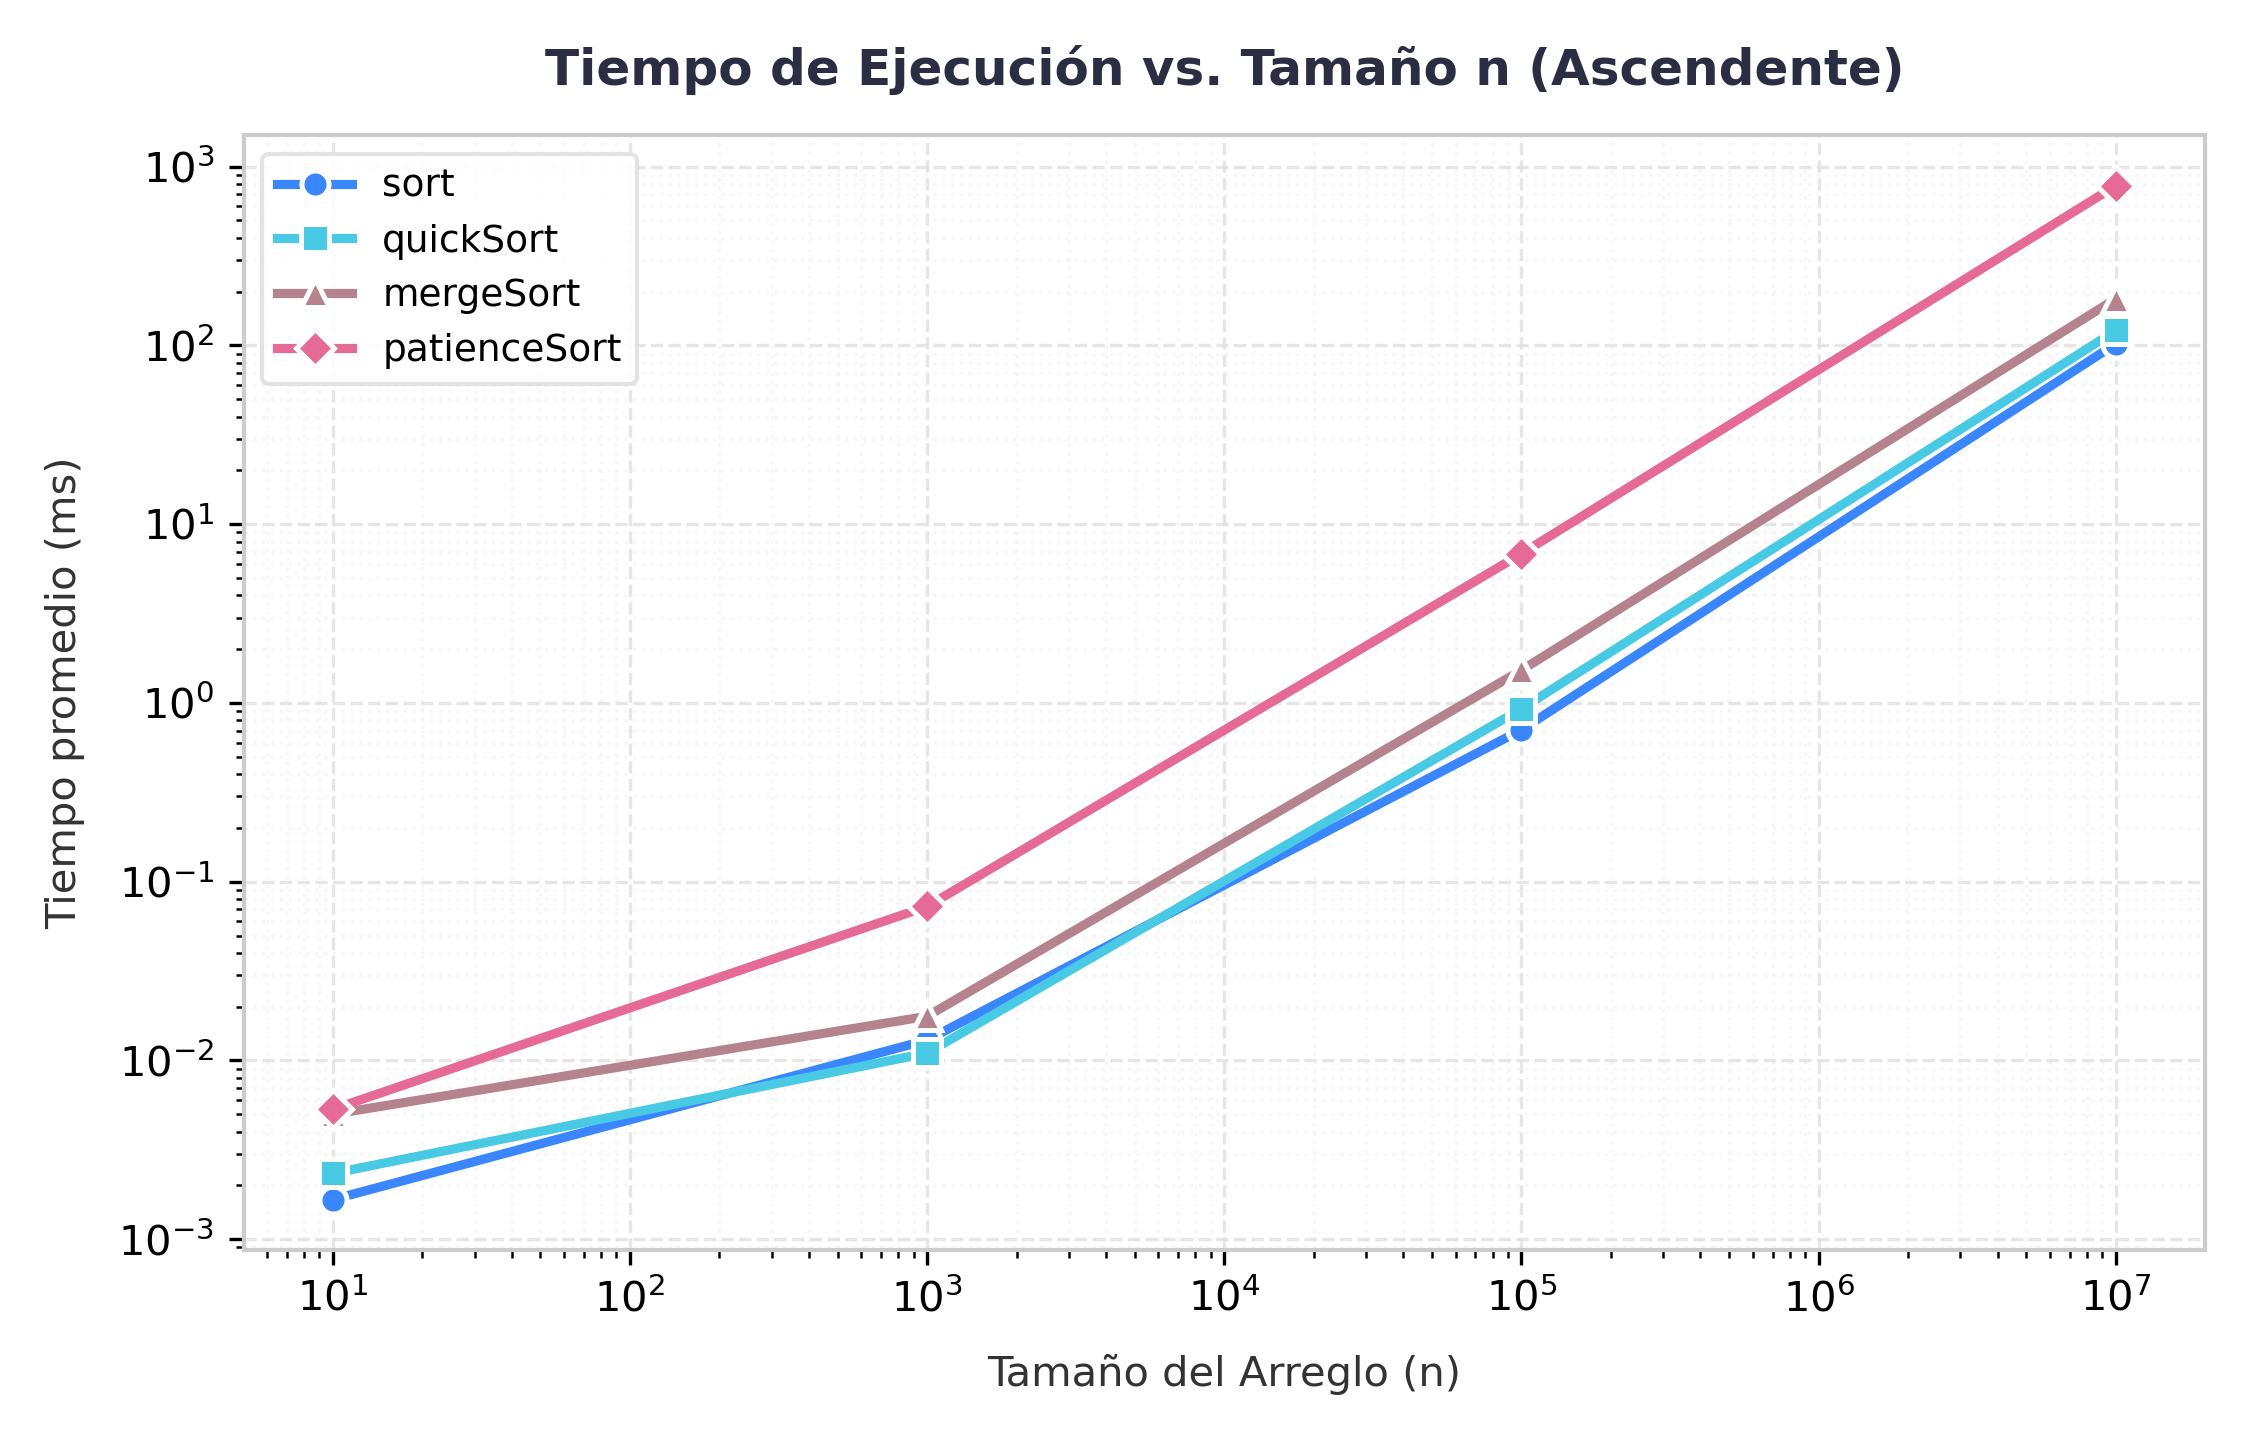
\includegraphics[width=0.48\linewidth]{../code/sorting/data/plots/tiempo_sorting_ascendente.png}%
    }
    \caption{Tiempo de ejecución promedio vs. tamaño $n$ para distintas distribuciones iniciales.}
    \label{fig:sort_time_distribuciones}
\end{figure}

Al evaluar las instancias aleatorias y ascendentes (\Cref{fig:sort_time_distribuciones}), los cuatro algoritmos presentan curvas con pendientes similares en escala log-log, confirmando que todos escalan según la familia $n \log n$. No obstante, \textsc{PatienceSort} se posiciona de manera constante como el algoritmo menos veloz. Esto se debe a que la dispersión y crecimiento de los elementos fuerza la creación de un número masivo de pilas ($p \approx n$), saturando la búsqueda binaria y encareciendo las operaciones en la cola de prioridad. En contraste, \textsc{QuickSort} y \textsc{sort} se mantienen como los más rápidos gracias a su naturaleza \emph{in-place}, la cual los hace mas rapidos al no tener que transferir datos a un arreglo auxiliar como hace \textsc{MergeSort}.

\begin{figure}[H]
    \centering
    \subfloat[Arreglos ordenados descendentemente.\label{fig:sort_time_descendente}]{%
        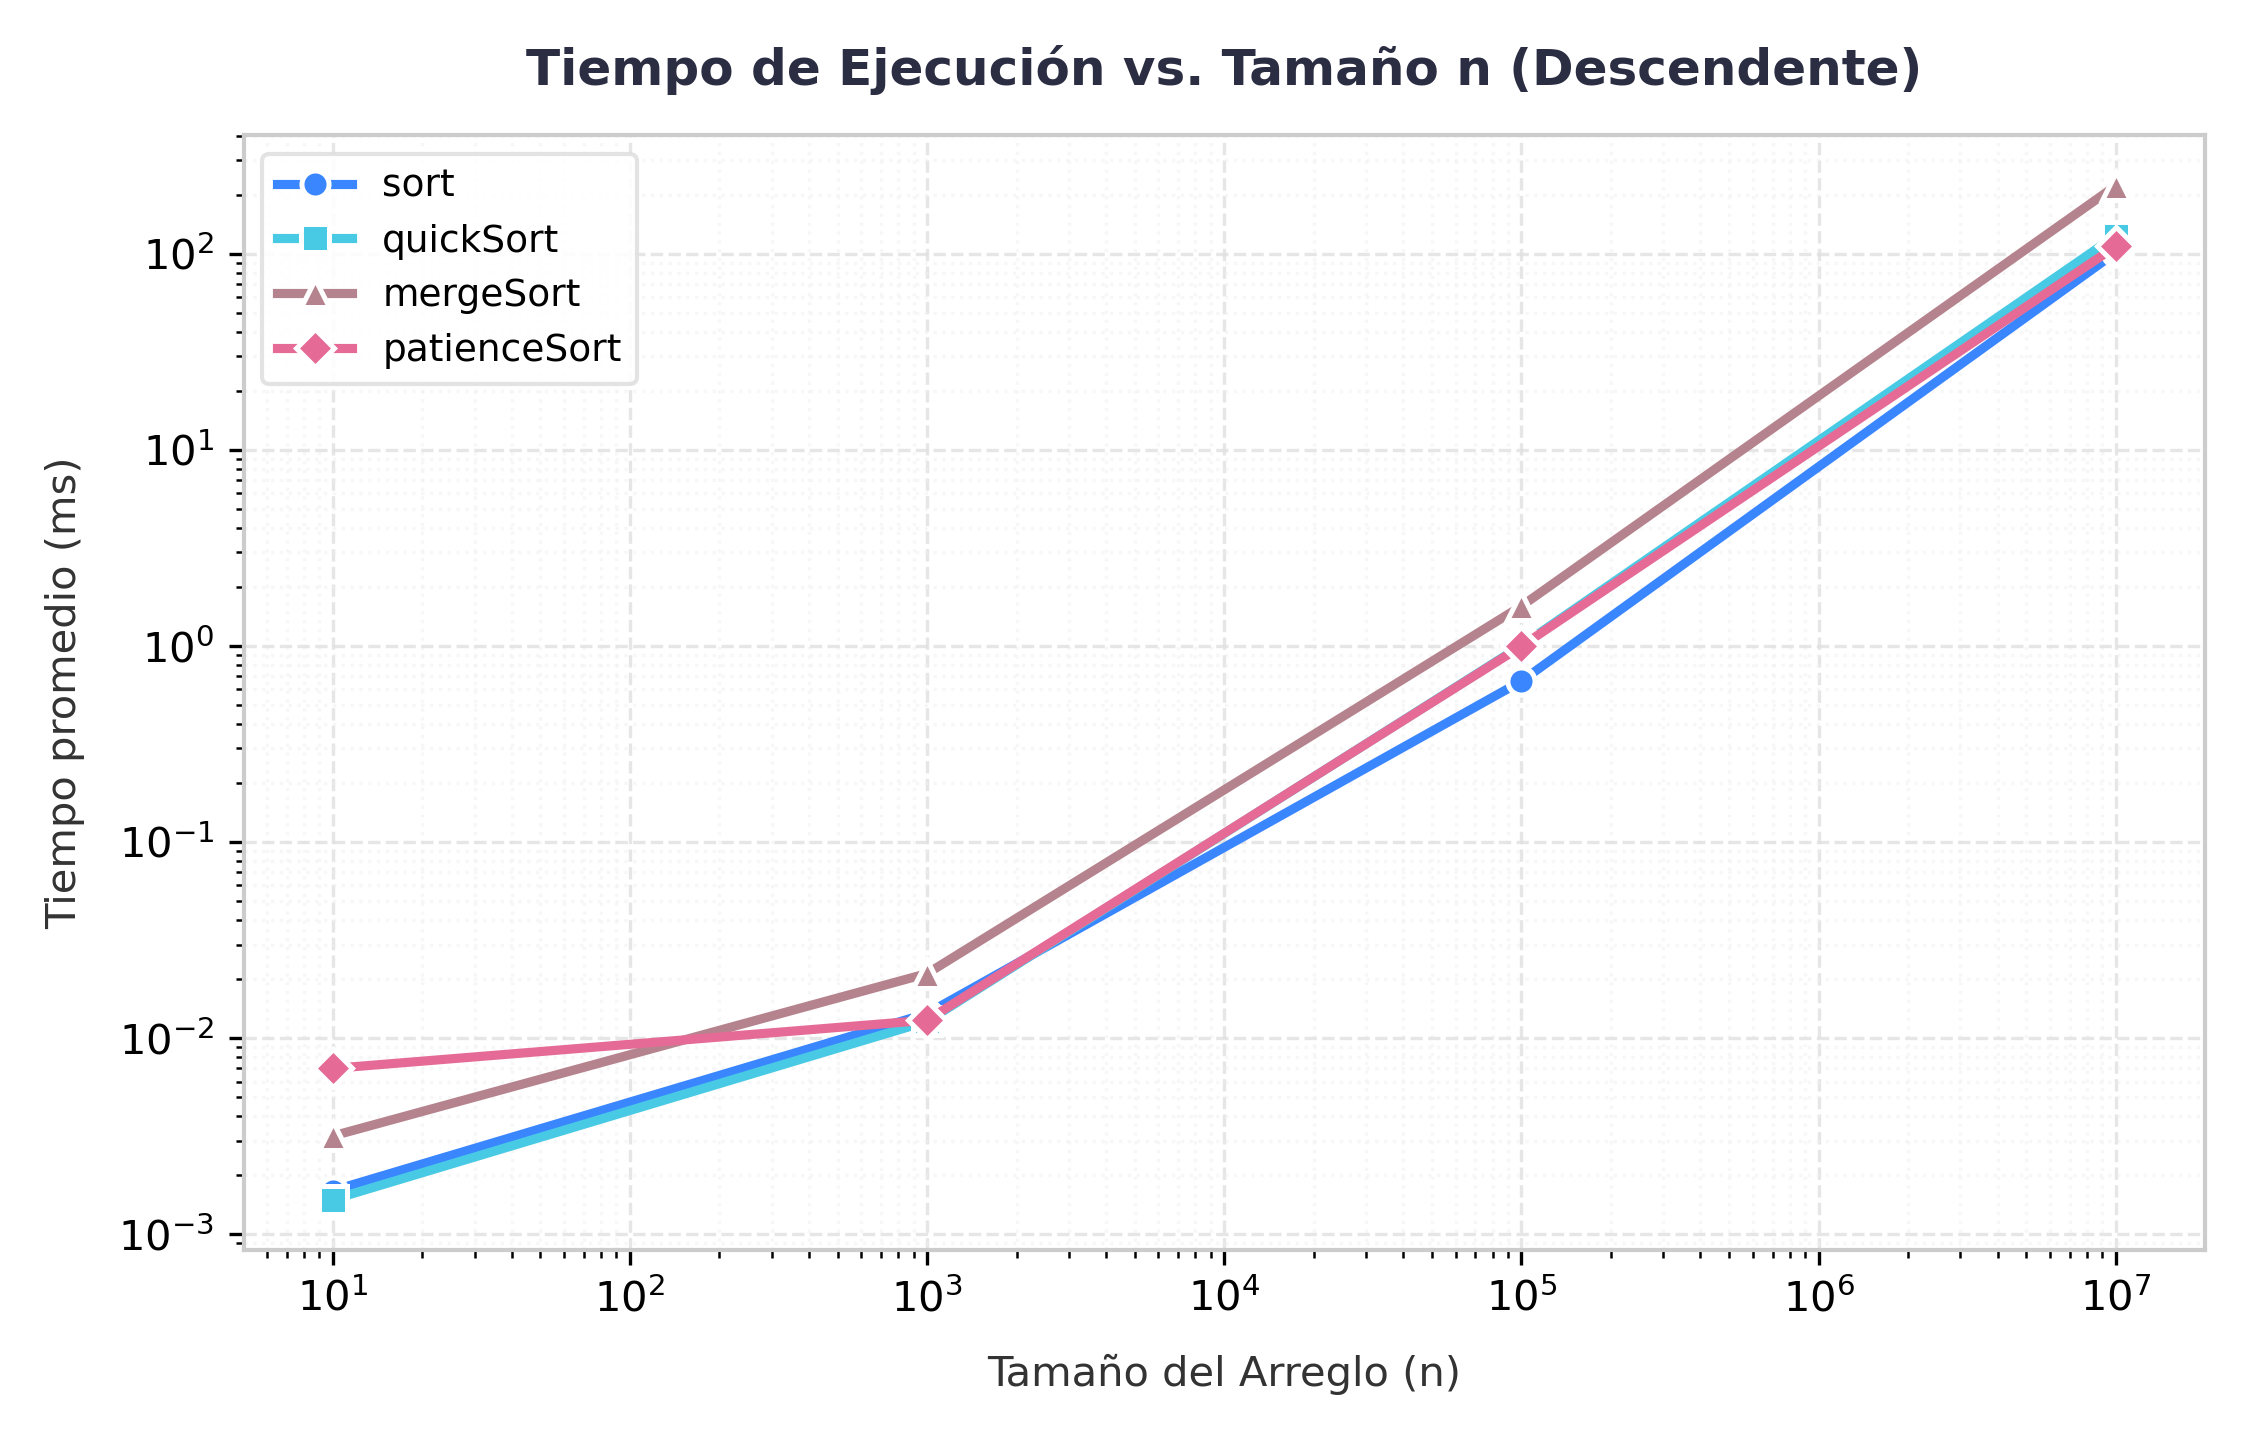
\includegraphics[width=0.48\linewidth]{../code/sorting/data/plots/tiempo_sorting_descendente.png}%
    }
    \hfill
    \subfloat[Entradas aleatorias en dominio $D_1 = \{0,\dots,9\}$.\label{fig:sort_time_d1}]{%
        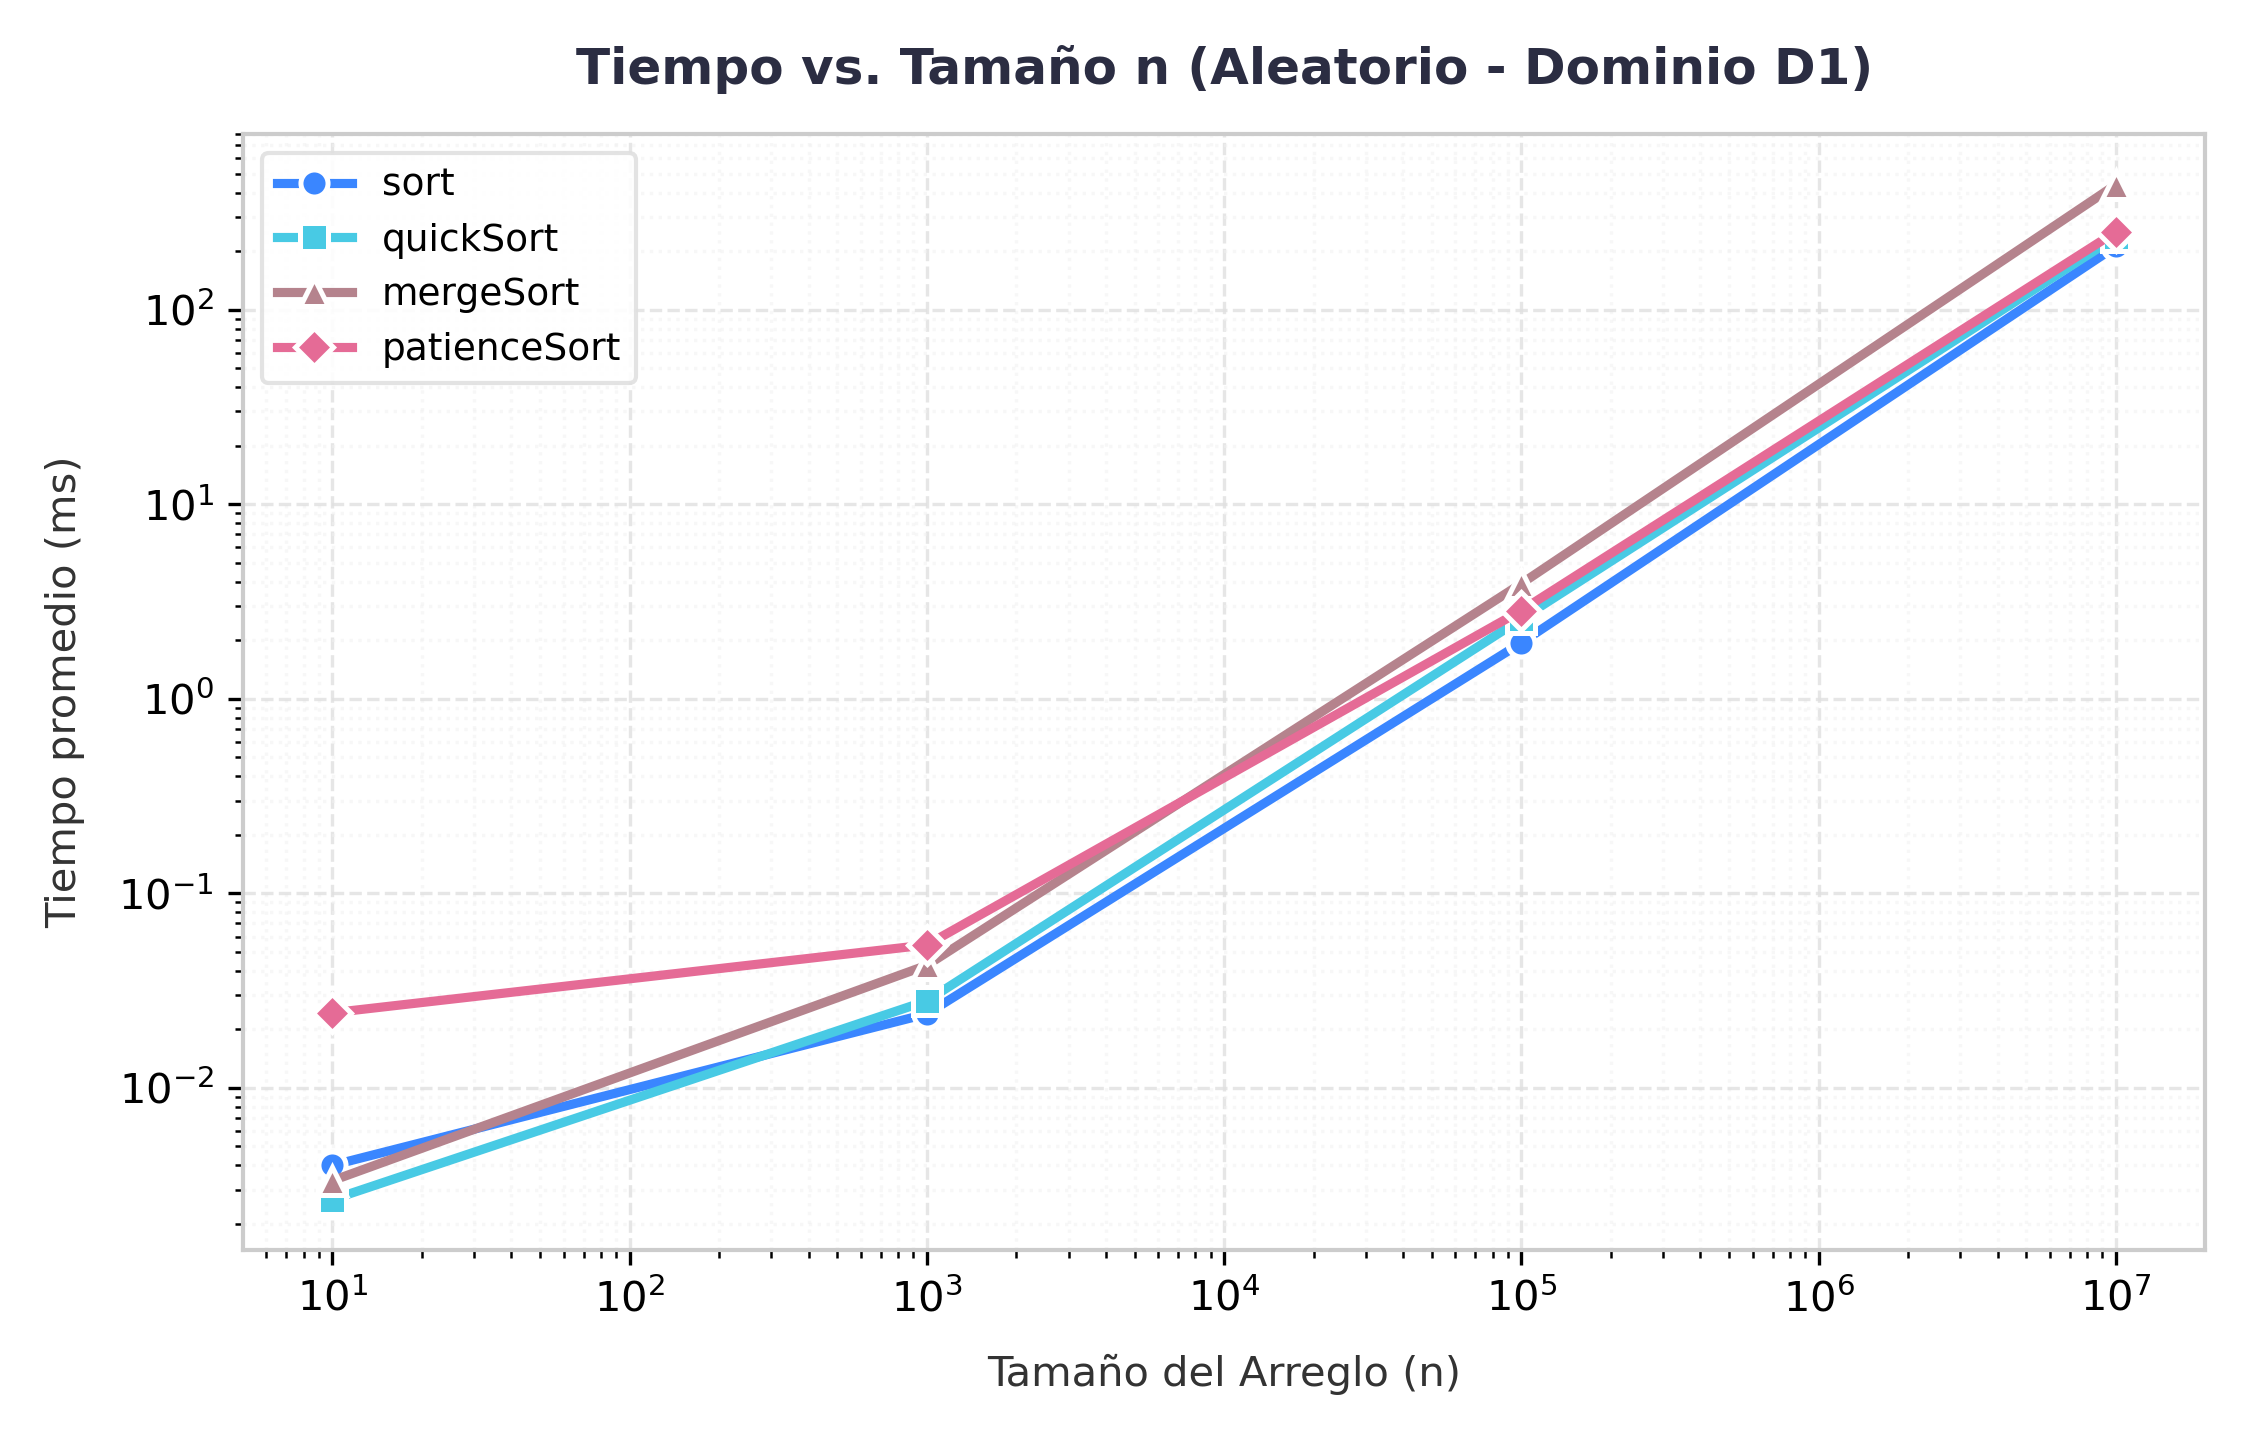
\includegraphics[width=0.48\linewidth]{../code/sorting/data/plots/tiempo_sorting_dominio_D1.png}%
    }
    \caption{Comportamiento adaptativo de los algoritmos de ordenamiento frente al caso favorable y a la variación del dominio numérico.}
    \label{fig:sort_time_adaptativo}
\end{figure}

La naturaleza adaptativa de \textsc{PatienceSort} se verifica empíricamente en la \Cref{fig:sort_time_descendente}. En arreglos con orden descendente, cada nuevo elemento resulta estrictamente menor que el tope anterior, acumulándose la totalidad de la entrada en una única pila ($p = 1$). Esto suprime el uso intensivo del heap y permite extraer la secuencia de forma lineal, logrando que la curva de \textsc{PatienceSort} descienda drásticamente hasta alcanzar la velocidad de los métodos \emph{in-place}, en concordancia con su mejor cota teórica $O(n)$. Por su parte, la \Cref{fig:sort_time_d1} demuestra el impacto del dominio: en $D_1$, al contar con solo diez valores posibles, la cantidad de pilas queda restringida a $p \le 10$, lo que aplana sustancialmente la curva de \textsc{PatienceSort} y lo sitúa notablemente más veloz que \textsc{MergeSort}.

\subsection{Memoria de Algoritmos de Multiplicación de Matrices}

Para el producto de matrices cuadradas de orden $n \times n$, \textsc{Naive} opera con una memoria auxiliar constante de $O(1)$, requiriendo únicamente el espacio cuadrático $\Theta(n^2)$ destinado a almacenar la matriz solución. En contraparte, \textsc{Strassen} aplica dividir y conquistar desglosando la matriz en cuatro cuadrantes de orden $n/2$ y generando siete matrices intermedias ($P_1 \dots P_7$) por cada nivel de llamada; aunque la convergencia de la serie espacial teórica mantiene una cota de $O(n^2)$, introduce una constante de asignación muy superior.

\begin{figure}[H]
    \centering
    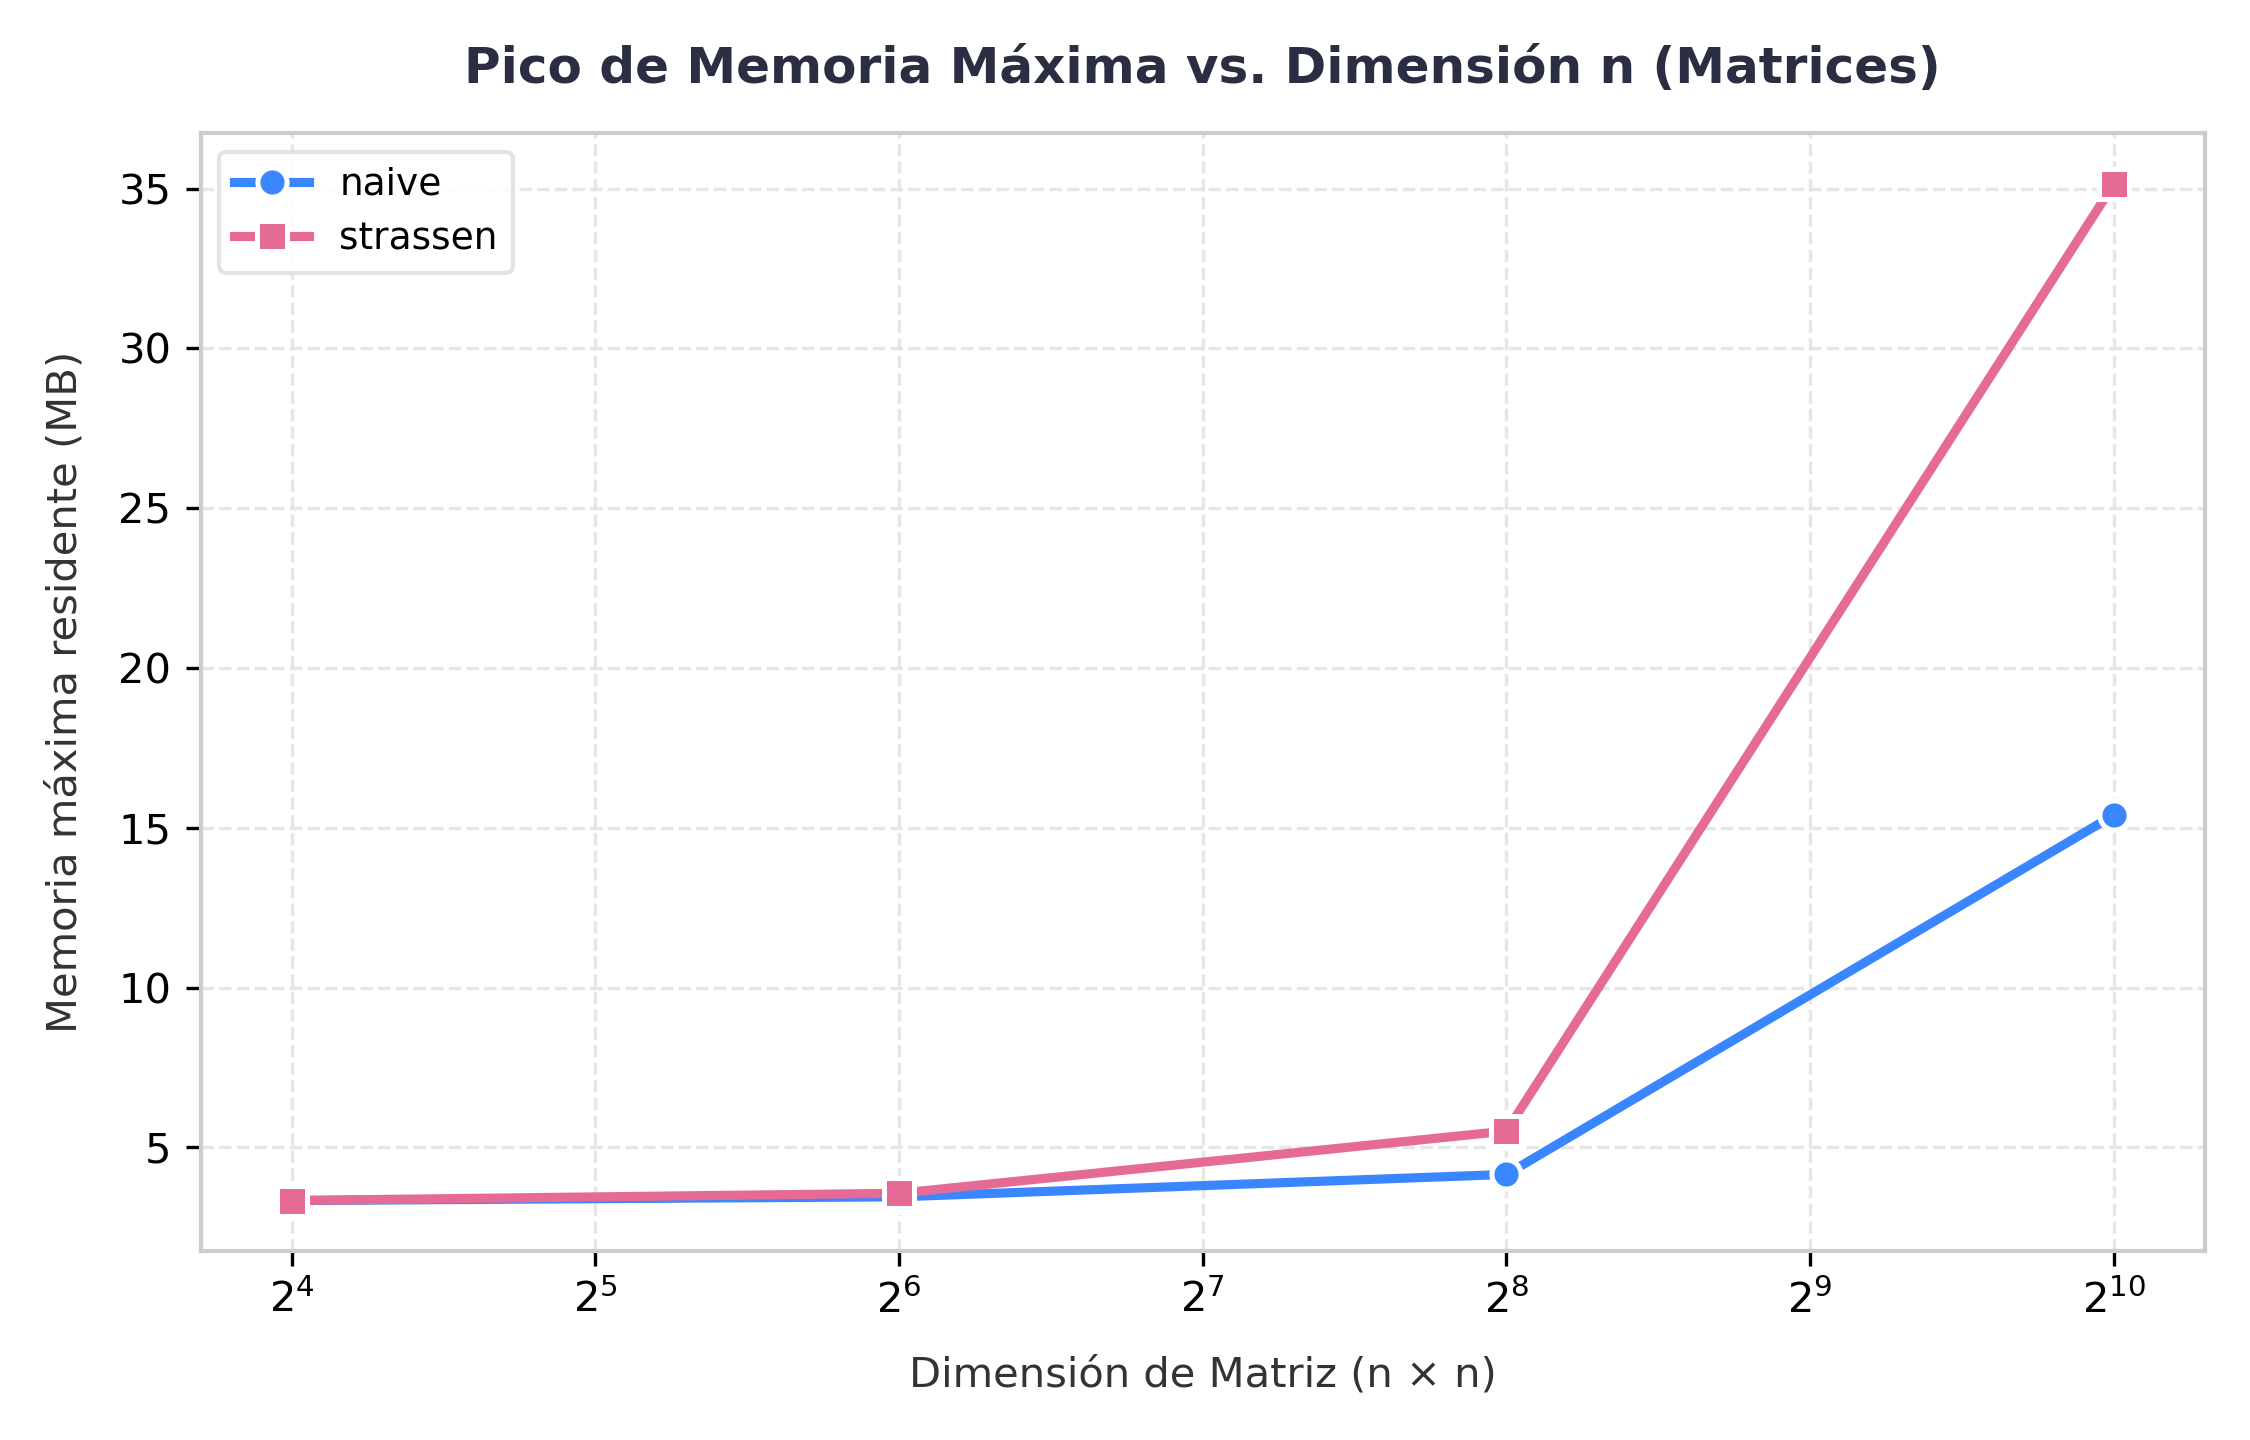
\includegraphics[width=0.72\linewidth]{../code/matrix_multiplication/data/plots/memoria_matrices.png}
    \caption{Pico de memoria máxima vs. dimensión $n$ en multiplicación de matrices.}
    \label{fig:matrix_mem}
\end{figure}

En la \Cref{fig:matrix_mem} se constata que \textsc{Strassen} utiliza considerablemente más memoria que \textsc{Naive}, incrementándose esta brecha conforme aumenta la dimensión $n$. Mientras que \textsc{Naive} exhibe un consumo plano y predecible al no demandar estructuras auxiliares durante el recorrido de sus bucles, \textsc{Strassen} acumula múltiples submatrices dinámicas creadas en el \emph{heap} durante la recursión, confirmando que las constantes ocultas de asignación dinámica dominan el consumo físico del sistema.

\subsection{Tiempo de Ejecución de Algoritmos de Multiplicación de Matrices}

Teóricamente, el método iterativo clásico \textsc{Naive} ejecuta tres bucles anidados con $n^3$ multiplicaciones escalares, fijando una cota estricta de $\Theta(n^3)$. Por su parte, la complejidad de \textsc{Strassen} se deduce a partir de su ecuación de recurrencia $T(n) = 7\,T(n/2) + \Theta(n^2)$, asociada a la ejecución de 7 productos recursivos y operaciones de adición/sustracción de bloques en tiempo cuadrático. Aplicando el Teorema Maestro, los parámetros $a = 7$ y $b = 2$ determinan el exponente crítico $\log_2 7 \approx 2.807$; dado que $f(n) = \Theta(n^2) = O(n^{\log_2 7 - \varepsilon})$ para $\varepsilon \approx 0.807$, rige el Caso 1, concluyendo una cota teórica asintótica de $\Theta(n^{\log_2 7}) \approx \Theta(n^{2.807})$.

\begin{figure}[H]
    \centering
    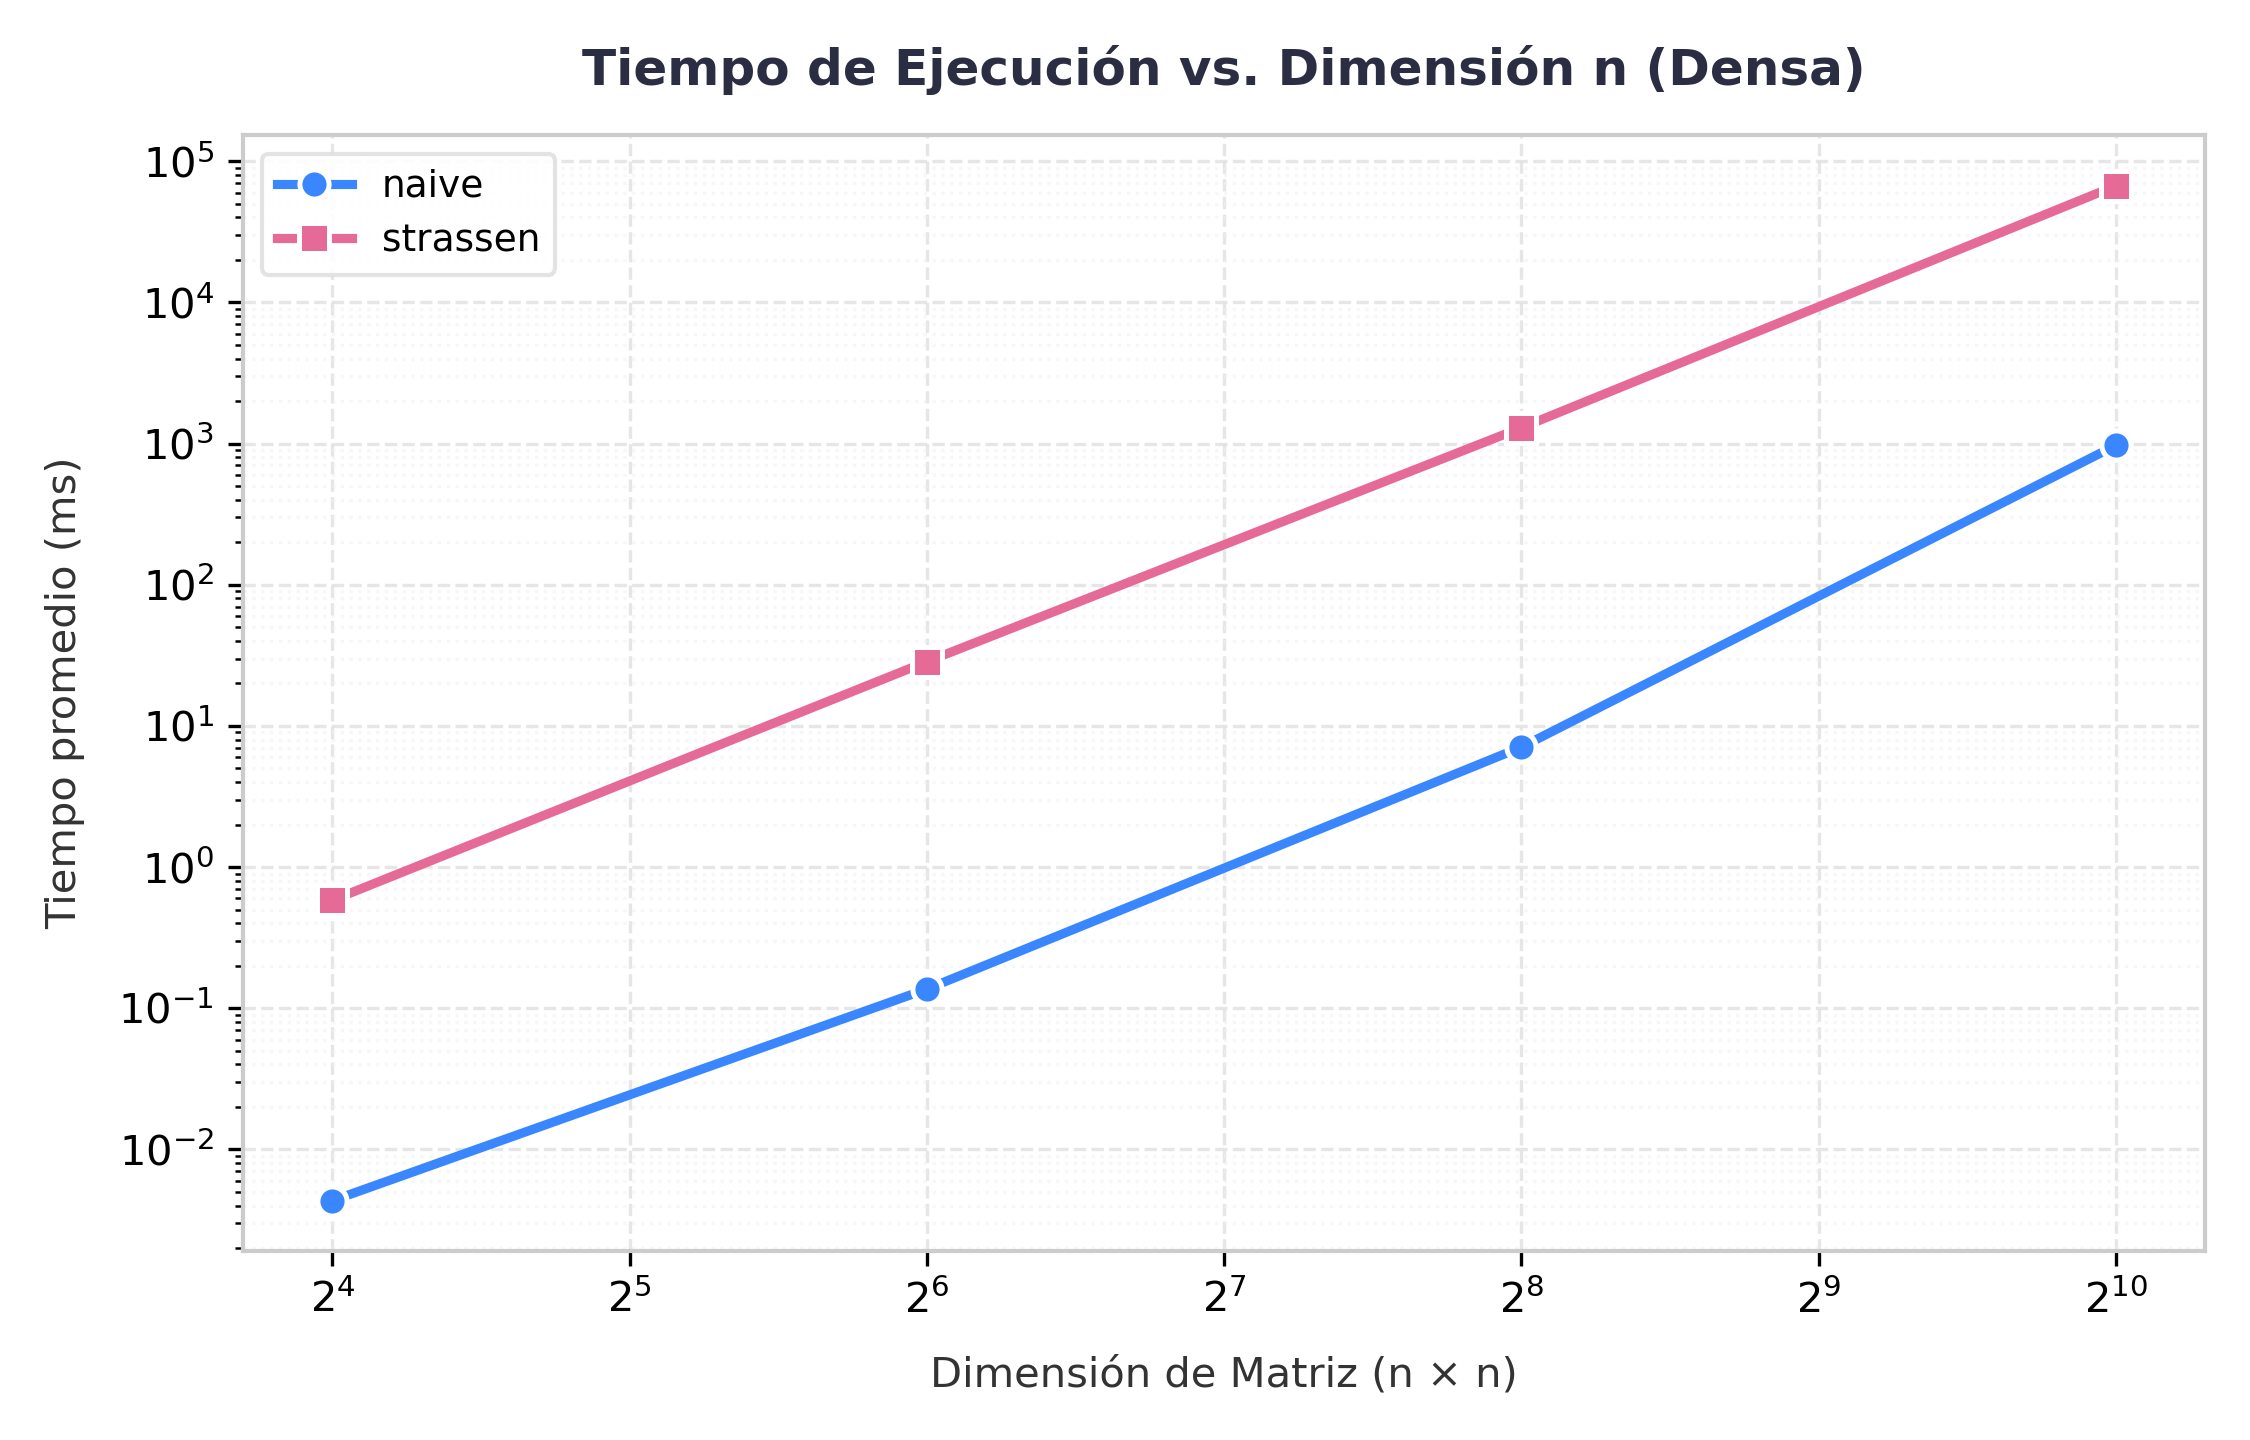
\includegraphics[width=0.72\linewidth]{../code/matrix_multiplication/data/plots/tiempo_matriz_densa.png}
    \caption{Tiempo de ejecución promedio vs. dimensión $n$ en matrices densas.}
    \label{fig:matrix_dense}
\end{figure}

A pesar de que la cota de \textsc{Strassen} ($n^{2.807}$) es asintóticamente inferior a la de \textsc{Naive} ($n^3$), en la \Cref{fig:matrix_dense} se observa que \textsc{Strassen} resulta menos eficiente en la práctica para las dimensiones evaluadas. Esto no invalida la teoría, sino que evidencia el impacto de las constantes multiplicativas omitidas por la notación asintótica. \textsc{Strassen} ahorra productos de submatrices a expensas de introducir numerosas sumas y restas intermedias, sumado a la sobrecarga fija de instanciar vectores en el \emph{heap} y apilar llamadas recursivas. Para dimensiones $n \le 1024$, este costo administrativo continuo supera el beneficio asintótico, permitiendo que la ejecución lineal y secuencial de bucles anidados en \textsc{Naive} aproveche mejor la caché y domine temporalmente en el hardware evaluado.